% -----------------------------*- LaTeX -*------------------------------
\documentclass[11pt]{report}
\usepackage{scribe_ds603}
\begin{document}


\scribe{Anilesh Bansal}		% required
\lecturenumber{4}			% required, must be a number
\lecturedate{8th August}		% required, omit year


\maketitle


% ----------------------------------------------------------------------

\section{Unsupervised Learning for Anomaly Detection}
Let $X \subseteq \Rbb ^d$ be the data space given by some task
or application sampled from a ground-truth distribution $\mathbb{P}^+$ with a corresponding pdf $p^+(x)$. We define a set of anomalies as 
\begin{align} \label{anomaly_set}
    A \Let \aset[\big]{\dcv \in \mathcal{X} \suchthat p^+(x) \leq \tau}, \tau \geq 0. 
\end{align}
Let $P$ be the ground-truth data-generating distribution
on data space $X \subseteq \Rbb ^d$ with corresponding density $p(x)$,
that is, the distribution that generates the observed data. For now, we assume that this data-generating distribution exactly matches the normal data distribution, that is,
$\mathbb{P} \equiv \mathbb{P}^+$ and $p \equiv p+$. This assumption is often invalid in
practice, of course, as the data-generating process might
be subject to noise or contamination. 

\subsection{Clustering Assumption}
We assume that there exists some threshold $\tau \geq 0$ such that
\begin{align}
    X \backslash A = \aset[\big]{x \in  \mathcal{X} \suchthat p^+(x)>\tau}
\end{align} is non-empty and small (in the Lebesgue measure sense, think volume). This does not imply that the full
support $supp(p^+) = \aset{x \in \mathcal{X} \suchthat p^+(x) > 0}$ of must be bounded; only that some high-density subset of
the support is bounded. A standard univariate Gaussian’s
support is the full real axis, for example, but approximately
95\% of its probability mass is contained in the interval
[-1.96, 1.96].

\subsection{Level Sets}
 The density level set of $\mathbb{P}$ for some threshold $\tau \geq 0$ is given by $C = \aset{x \in X \suchthat p(x) > \tau}$. 
 
For some fixed level $\alpha \in [0, 1]$, the $\alpha$-density level set $C_\alpha$ of
distribution $\mathbb{P}$ is then defined as the smallest density level
set C that has a probability of at least $1 - \alpha$ under $\mathbb{P}$, that is,
\begin{align}
    C_\alpha &= \mathop{\arg\!\inf}_{C} \aset{\mu(C) \suchthat \mathbb{P}(C) \geq 1 - \alpha} \nonumber\\
     &= \aset{x \in \mathbb{X} \suchthat p(x) > \tau_\alpha}
\end{align}
where $\tau_\alpha \geq 0$ denotes the corresponding threshold and
$\mu$ is typically the Lebesgue measure.

Given a level set \( C_\alpha \), we can define a corresponding
threshold anomaly detector \( c_\alpha : \mathcal{X} \rightarrow \{ \pm 1 \} \) as

\begin{align}
    c_\alpha(x) =
    \begin{cases}
    +1, & \text{if } x \in C_\alpha \\
    -1, & \text{if } x \notin C_\alpha
    \end{cases}
\end{align}
\begin{figure}
    \centering
    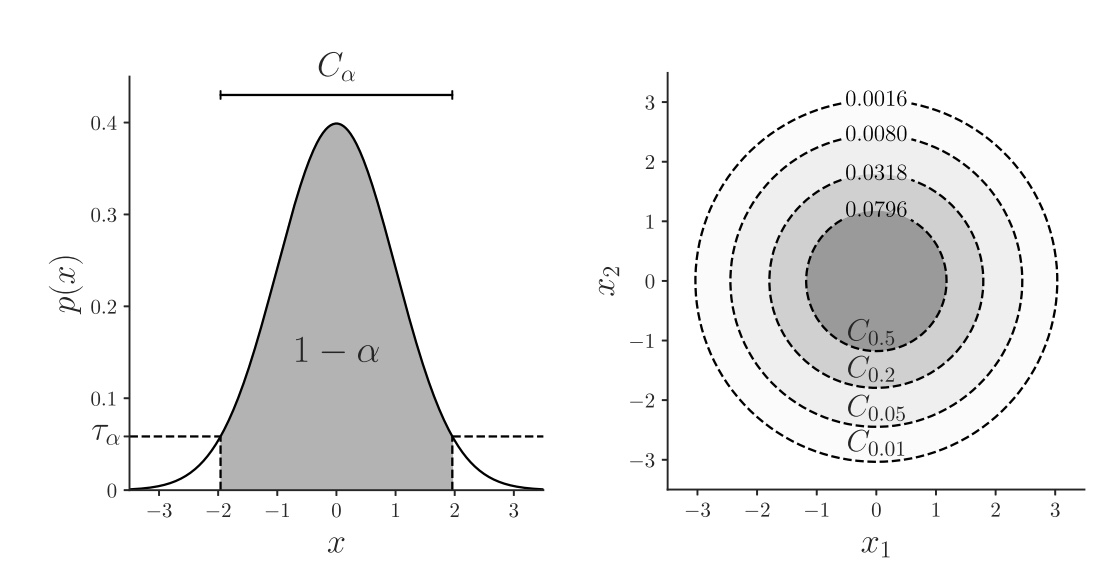
\includegraphics[width=0.5\linewidth]{images/levelset.jpeg}
    \caption{Illustration of the $\alpha$-density level sets $C_\alpha$ with threshold
$\tau_\alpha$ for a univariate (left) and bivariate (right) standard Gaussian
distribution. \cite{ruff2020unifying}}
    \label{fig:placeholder}
\end{figure}

Thus if $c_\alpha(x)$ is -1, we label the point x as an anomaly. Thus our task of finding anomalies reduces to the task of finding or estimating the underlying distribution p.

\section{Estimating the distribution p}
\subsection{Parametric Vs Non-Parametric density estimation} One can have priors about the distribution $p$ and try to get estimates of parameter $\theta$ such that $p_\theta(x)$ is maximized.

    For example, if it's known that samples are from a gaussian with unknown mean and known variance, $\mathcal{N}(\mu, \sigma)$, we know that $\hat{\mu}
    = \frac{\sum _{i=1} ^n x_i}{n}$ is an unbiased estimator of the true mean $\mu$. In fact, it can be shown that it is the uniformly minimum-variance unbiased estimator (UMVUE) i.e. an unbiased estimator that has lower variance than any other unbiased estimator for all possible values of the parameter.

    After we have an estimate of $\theta$ i.e. $\hat{\theta} = \hat{\mu}$ , we can use it for estimating p and finding outliers. 

    However, it's not necessary that the underlying distribution can be represented through a family of distributions and parameters. In this case, it's called a non-parametric density estimation. 
    
Thus in parametric, the $\theta$ to be estimated is finite-dimensional. In non-parametric, $\theta$ is infinite-dimensional. As a concrete example of non-parametric family of distributions, consider the family of all measurable functions, i.e. $p^+(x)$ can be any measurable density $f: \Rbb^d \ra \Rbb$ and $\theta \equiv f$ and $\Theta \equiv \mathcal{F}$ (space of all measurable functions). In this case parameter estimation is not possible, and we do kernel density estimation instead.

\subsection{Kernel Density Estimation}
Denote by $B(x, h)$ a ball of sze h centered around x. If $p^+(x)$ changes slowly around $B(x,h)$ i.e. 
\begin{align}
    \mathbb{P}(B(x,h)) = \int _{x \in B(x,h)} p^+(x)dx \approx p^+(x) \int _{x \in B(x,h)} dx = p^+(x) \mu(B(x,h))
\end{align}
Thus we can get a local density estimate of $p^+(x)$ that depends on the choice of $h$ as
\begin{align}
    \hat{p}_h^+(x) = \frac{\hat{\mathbb{P}}(B(x,h)}{\mu(B(x,h))}
\end{align}
where $\hat{\mathbb{P}}$ estimates the probability in a region. For example if we define $\hat{\mathbb{P}}$ as
\begin{align}
    \hat{\mathbb{P}}(B(x,h)) &= \frac{1}{n} \sum _{i=1} ^n \mathbbm{1}\left[ x_i \in B(x,h)\right]\\
    \implies \hat{p}_h^+(x) &= \frac{1}{n \mu(B(x,h))}\sum _{i=1} ^n \mathbbm{1}\left[ \norm{x - x_i} \leq h\right] \nonumber\\
    &= \frac{1}{nh^dV}\sum _{i=1} ^n \mathbbm{1}\left[ \frac{\norm{x - x_i}}{h} \leq 1\right] \tag*{\text{($V_d=$volume for $d$-dimensional ball of unit radius)}} \nonumber\\
    &= \frac{1}{nh^d}\sum _{i=1} ^n K\left(\frac{\norm{x - x_i}}{h}\right) \tag*{\text{(Using kernel function $K(u) = \frac{\mathbbm{1}[\norm{u} \leq 1]}{V_d}$)}} \nonumber\\
\end{align}
Here we ended up using a Box-Kernel, which is defined as above. Instead, one can also use other kernels like Gaussian $(K(u) = \frac{1}{Z} \exp(-\norm{u}^2/2))$. In fact we can use any $K: \Rbb^d \ra \Rbb$ s.t. $\int _{\Rbb^d} K(u)du = 1$. 

We call $h$ as the bandwidth, and the choice of $h$ leads to an obvious bias-variance tradeoff - if $h$ is too small $\implies$ smaller bias, however a larger variance since number of points used for estimation are smaller. If $h$ is too large, this variance reduces, however, then $\hat{p}_h^+(x)$ is biased. 

But if we choose $h$ appropriately, it can be shown that $\hat{p}_h^+(x)$ converges to true $p(x)$. Chen 2017 \cite{Chen2017-ns} considers the following three errors and gives theoretical convergence rates based on the the choice of $h$. \begin{enumerate}
    \item pointwise error i.e. $\hat{p}_h^+(x) - p(x)$
    \item uniform error i.e. $\sup\limits_x \abs{\hat{p}_h^+(x) - p(x)}$ 
    \item Mean Integrated Square Error (MISE) i.e. $\int \mathbb{E}\left[\hat{p}_h^+(x) - p(x)\right]^2dx$
\end{enumerate} 

\subsection{Plug-in approach to get level set estimates}
We can get an estimate of the level sets as follows 
\begin{align}
    \hat{C}_\alpha = \aset{x \in \mathcal{X} \suchthat \hat{p}_h^+(x) > \lambda}
\end{align} such that $\hat{p}_h^+(x) > \lambda$ captures some sufficient probability. However, this is a very roundabout approach of selecting outliers since we first need the density and this generates quantiles for all values of $\alpha$, which is too overkill for the task of finding outliers. 

Instead can we do a Frequentist approach and find a function $f$ that is +1 over some set $C_\alpha$ and -1 everywhere else. This is similar in idealogy to just using a discriminator instead of a generative model for tasks like classification - you don't want to regenerate entire $x$ if the final task is just classification.

\section{Support Vector Data Description (SVDD)}
Given $x_1, x_2, \cdots, x_n \in \mathcal{X}$, consider the following constrained optimization problem:
\begin{align}
\min_{R, \mathbf{c}, \boldsymbol{\gamma}} \quad & R^2 + \frac{1}{\nu n} \sum_{i=1}^{n} \gamma_i \\
\text{subject to} \quad & \|\mathbf{x}_i - \mathbf{c} \|^2 \leq R^2 + \gamma_i, 
&& i = 1, \ldots, n, \label{svdd-const1} \\
& \gamma_i \geq 0, 
&& i = 1, \ldots, n, \label{svdd-const2}
\end{align}
 Where does this optimization problem arise from? We can think of $\boldsymbol{c}, R$ as the center and radius of an enclosing ball, and any test input $\boldsymbol{x}$ that lies outside this ball is deemed an outlier. 
$$\norm{\boldsymbol{x} - \boldsymbol{c}}^2 > R^2$$
Here $\nu_n$ is a hyperparameter that controls the impact of slack variables $\gamma$ - intuitively it is equivalent to the fraction of points outside the enclosing ball. 

We'll now look at what loss function the above problem actually minimizes and under what conditions. 

\subsection{Deriving the sphere optimization problem}
Ultimately, we want a solution that minimizes the following loss function
\begin{align}
    \arg\!\min_h L(h) 
    = \arg\!\min_h \mathbb{E}\limits_{\boldsymbol{x} \sim \mathbb{P}^+} \left[ l(h(\boldsymbol{x}), 1) \right] + \mathbb{E}\limits_{\boldsymbol{x} \sim \mathbb{P}^-} \left[ l(h(\boldsymbol{x}), -1) \right]
\end{align}
Since we cannot get any samples from $\mathbb{P^-}$, we typically add a regularizer to the loss function to account for the latter term. Typically the regularizer is a norm constraint (say L1 or L2 norm) on the hypothesis $h$ i.e.
$$\hat{L_R}(h) = \frac{1}{n}\sum _{i=1} ^n l(h(\boldsymbol{x}, 1) + R(h)$$

To get to the sphere optimization problem, we make the following assumptions - 
\begin{enumerate}
    \item Assumption 1: Define $f_\theta(\boldsymbol{x}) = R^2 - \norm{\boldsymbol{x} - \boldsymbol{c}}^2$ and $h_\theta(\boldsymbol{x}) = sign(f_\theta(\boldsymbol{x}))$ where the parameter $\theta = (R, \boldsymbol{c})$.  Basically we deem $\boldsymbol{x}$ as an outlier ($h_\theta = -1$) whenever $\boldsymbol{x}$ is outside the enclosing ball. And we also enforce the score $f_\theta$ drops linearly with squared norm of distance from center of the ball. 
    \item Assumption 2:Loss function is the shifted, cost-weighted hinge loss:
        \[
        \ell(h_\theta(\boldsymbol{x}), y) = 
        \begin{cases}
        \frac{1}{1 + \nu} \max(0, -f_\theta(\boldsymbol{x})) & y = +1 \\
        \frac{\nu}{1 + \nu} \max(0, f_\theta(\boldsymbol{x})) & y = -1
        \end{cases}
        \]
    \item $\mathbb{P}^- = \text{Unif}(\mathcal{X})$ (this inherently assumes $\mathcal{X}$ to be bounded )
\end{enumerate}
Under these assumptions, we can rewrite $L(h_\theta)$ or equivalently $L(\theta)$ as 
\[
L(\theta) = \mathbb{E}_{\boldsymbol{x} \sim \mathbb{P}^+} \left[ \frac{1}{1 + \nu} \max\left(0, \|\boldsymbol{x} - \boldsymbol{c}\|^2 - R^2\right) \right] 
\rightarrow L_+(\theta)
\]
\[
\quad + \mathbb{E}_{\boldsymbol{x} \sim \mathbb{P}^-} \left[ \frac{\nu}{1 + \nu} \max\left(0, R^2 - \|\boldsymbol{x} - \boldsymbol{c}\|^2 \right) \right] 
\rightarrow L_-(\theta)
\]
\text{Under Assumption 3:}
\[ L_{-}(\theta) = 
\mathbb{E}_{\boldsymbol{x} \sim \mathbb{P}^-} \left[ \frac{\nu}{1+\nu} \max(0, R^2 - \|\boldsymbol{x} - \boldsymbol{c}\|^2) \right]
= \frac{\nu}{1+\nu} \int \max(0, R^2 - \|\boldsymbol{x} - \boldsymbol{c}\|^2) \, d\mathbb{P}^-(\boldsymbol{x})
\]
\[
= \frac{\nu}{1+\nu} \cdot \frac{1}{\mu(\mathcal{X})} \int \max(0, R^2 - \|\boldsymbol{x} - \boldsymbol{c}\|^2) \, d\mu(\boldsymbol{x})
\]
\[
\leq \frac{\nu}{1+\nu} \cdot \frac{1}{\mu(\mathcal{X})} \int R^2 \, d\mu(\boldsymbol{x})
\]
\[
= \frac{\nu}{1+\nu} \cdot \frac{1}{\mu(\mathcal{X})} \cdot \left( \mu(B_R(\boldsymbol{c})) \cdot R^2 \right)
\]
\[
= \frac{\nu}{1+\nu} R^2 \cdot \frac{\mu(B_R(\boldsymbol{c})}{\mu(\mathcal{X})}
\]
\[
\Rightarrow L^-(\theta) \leq \frac{\nu}{1+\nu} R^2
\]

\[
\Rightarrow L(\theta) \leq L^+(\theta) + \frac{\nu}{1+\nu} R^2
\]


Setting:
\[
\gamma_i = \max(0, \|\boldsymbol{x}_i - \boldsymbol{c}\|^2 - R^2)
\Rightarrow
L^+(\theta) = \frac{1}{(1+\nu)n}\sum _{i=1} ^n \gamma_i
\]

\[
\implies L(\theta) \leq \frac{\nu}{1+\nu}\left[ R^2 + \frac{1}{\nu n} \sum_{i=1}^n \gamma_i \right]
\]

\text{Thus minimizing the upper bound on the loss, we recover the sphere optimization problem we started with}
\[
L_S(\theta) = R^2 + \frac{1}{\alpha n} \sum_i \gamma_i \quad \text{s.t. } \gamma_i \geq 0,\quad \gamma_i \geq \|\boldsymbol{x}_i - \boldsymbol{c}\|^2 - R^2
\]

\section{Solving the problem - Lagrangian Dual}
Let us briefly recall some definitions (see \cite[Ch.~5]{boyd2004convex}).  
For a primal problem
\begin{align*}
\min_{\mathbf{x}} \quad & f_0(\mathbf{x}) \\
\text{s.t.} \quad & f_i(\mathbf{x}) \leq 0, \quad i=1,\dots,m,
\end{align*}
the \emph{Lagrangian} is
\[
\mathcal{L}(\mathbf{x}, \boldsymbol{\alpha}) = f_0(\mathbf{x}) + \sum_{i=1}^m \alpha_i f_i(\mathbf{x}),
\]
with dual variables $\alpha_i \geq 0$.  
The \emph{dual function} is
\[
g(\boldsymbol{\alpha}) = \inf_{\mathbf{x}} \, \mathcal{L}(\mathbf{x}, \boldsymbol{\alpha}),
\]
and the \emph{dual problem} is:
\[
g^* = \sup_{\boldsymbol{\alpha} \ge 0} \; g(\boldsymbol{\alpha}).
\]
Formally, the dual optimum should be written with $\sup$ rather than $\max$, 
since in general the maximum may not be attained. In the SVDD case, however, 
strong duality ensures that the supremum is attained, so it is also valid to write
\[
g^* = \max_{\boldsymbol{\alpha} \ge 0} \; g(\boldsymbol{\alpha}).
\]

By \textbf{weak duality}, the dual optimum is always a lower bound to the primal optimum:
\[
g^* \le f_0(x^*).
\]

\subsection{Strong Duality}
For convex optimization problems satisfying Slater's condition (strict feasibility), \emph{strong duality} holds \cite[Section~5.3]{boyd2004convex}.  
This means the optimal primal and dual objective values coincide:
\[
g^\star = f_0(x^\star)
\]
Moreover, the optimal primal and dual variables correspond to a \emph{saddle point} of the Lagrangian, i.e.,
\[
\mathcal{L}(x^\star, \boldsymbol{\alpha}) \;\le\; \mathcal{L}(x^\star, \boldsymbol{\alpha}^\star) 
\;\le\; \mathcal{L}(x, \boldsymbol{\alpha}^\star), 
\quad \forall x, \; \forall \boldsymbol{\alpha} \ge 0,
\]
which means that $\mathcal{L}$ is minimized in $x$ at $x^\star$ and maximized in $\boldsymbol{\alpha}$ at $\boldsymbol{\alpha}^\star$.  
Equivalently, strong duality ensures the min–max equality:
\[
\inf_x \sup_{\boldsymbol{\alpha} \ge 0} \mathcal{L}(x,\boldsymbol{\alpha})
\;=\;
\sup_{\boldsymbol{\alpha} \ge 0} \inf_x \mathcal{L}(x,\boldsymbol{\alpha}).
\]

\subsection{Karush–Kuhn–Tucker (KKT) Conditions}
For convex, differentiable objectives and constraints, the following KKT conditions must hold for optimal primal variables $\theta^\star$ and optimal dual variables $(\lambda^\star, \mu^\star)$:
\begin{enumerate}
    \item \textbf{Primal feasibility:} All inequality and equality constraints are satisfied.
    \item \textbf{Dual feasibility:} $\lambda^\star \geq 0$ for all inequality constraints.
    \item \textbf{Complementary slackness:} For any inequality constraint $g_i(\theta) \leq 0$,
    \[
    \lambda_i^\star g_i(\theta^\star) = 0.
    \]
    \item \textbf{Stationarity:} The gradient of the Lagrangian with respect to $\theta$ vanishes:
    \[
    \nabla_\theta \mathcal{L}(\theta^\star, \lambda^\star, \mu^\star) = 0.
    \]
\end{enumerate}

\subsection{Application to SVDD}
The SVDD primal problem is:
\begin{align}
\min_{R, \mathbf{c}, \boldsymbol{\gamma}} \quad & R^2 + \frac{1}{\nu n} \sum_{i=1}^{n} \gamma_i \label{svdd-primal} \\
\text{subject to} \quad 
& \|\mathbf{x}_i - \mathbf{c} \|^2 - R^2 - \gamma_i \leq 0, 
&& i = 1, \ldots, n, \label{svdd-const1} \\
& -\gamma_i \leq 0, 
&& i = 1, \ldots, n. \label{svdd-const2}
\end{align}

\textbf{HW:} Verify that the SVDD primal problem is convex in $(R, c, \gamma)$ and satisfies the Slater's conditions for strong duality. \cite{chang2013svdd} \\

We form the Lagrangian by introducing multipliers $\alpha_i \geq 0$ for \eqref{svdd-const1} and $\beta_i \geq 0$ for \eqref{svdd-const2}:
\begin{align}
\mathcal{L}(R, \mathbf{c}, \boldsymbol{\gamma}, \boldsymbol{\alpha}, \boldsymbol{\beta}) 
= & R^2 + \frac{1}{\nu n} \sum_{i=1}^n \gamma_i \nonumber \\
& + \sum_{i=1}^n \alpha_i \left( \|\mathbf{x}_i - \mathbf{c} \|^2 - R^2 - \gamma_i \right) 
- \sum_{i=1}^n \beta_i \gamma_i.
\end{align}

\paragraph{Stationarity conditions:}
Taking derivatives and setting to zero:
\begin{align}
\frac{\partial \mathcal{L}}{\partial R} & : \quad 2R - 2R \sum_{i=1}^n \alpha_i = 0 
\quad \Rightarrow \quad \sum_{i=1}^n \alpha_i = 1, \\
\frac{\partial \mathcal{L}}{\partial \mathbf{c}} & : \quad -2 \sum_{i=1}^n \alpha_i (\mathbf{x}_i - \mathbf{c}) = 0
\quad \Rightarrow \quad \mathbf{c} = \sum_{i=1}^n \alpha_i \mathbf{x}_i, \\
\frac{\partial \mathcal{L}}{\partial \gamma_i} & : \quad \frac{1}{\nu n} - \alpha_i - \beta_i = 0
\quad \Rightarrow \quad \alpha_i \leq \frac{1}{\nu n}.
\end{align}

\paragraph{Dual problem:}
Substituting these into the Lagrangian yields the dual:
\begin{align}
\max_{\boldsymbol{\alpha}} \quad & 
\sum_{i=1}^n \alpha_i \mathbf{x}_i^\top \mathbf{x}_i 
- \sum_{i=1}^n \sum_{j=1}^n \alpha_i \alpha_j \mathbf{x}_i^\top \mathbf{x}_j \\
\text{subject to} \quad & 
\sum_{i=1}^n \alpha_i = 1, \\
& 0 \leq \alpha_i \leq \frac{1}{\nu n}.
\end{align}

Note that in this case we can easily solve the dual problem and get the value of the center as a linear combination of the input vectors $\boldsymbol{x_i}$
\[\mathbf{c} = \sum_{i=1}^n \alpha_i \mathbf{x}_i,\]
\textbf{HW: }Complete the proof of deriving the dual problem from the primal problem

\subsection{Complementary Slackness for SVDD}
At the optimum:
\begin{align}
\alpha_i \left( \|\mathbf{x}_i - \mathbf{c} \|^2 - R^2 - \gamma_i \right) &= 0, \\
\beta_i \gamma_i &= 0.
\end{align}
These help identify the \emph{support vectors} that lie exactly on the boundary of the enclosing ball.

\subsection{Other Feature Spaces and the Kernel Trick}

So far, everything has been formulated in the original input space 
$\mathbb{R}^d$, using the linear feature map
\[
\phi(\mathbf{x}) = \mathbf{x}.
\]
This corresponds to the kernel
\[
k(\mathbf{x}, \mathbf{x}') = \langle \mathbf{x}, \mathbf{x}' \rangle.
\]

\noindent
\textbf{Generalization:}  
Consider a feature map
\[
\phi: \mathbb{R}^d \to \mathbb{R}^p,
\]
where $p$ can be much larger than $d$, possibly infinite. Then, any 
$\mathbf{x}$ can be mapped to $\phi(\mathbf{x})$, and the SVDD formulation 
can be applied in this feature space.

Instead of explicitly computing $\phi(\mathbf{x})$, we can use the 
\emph{kernel trick}. That is, we choose a kernel function
\[
\tilde{k}(\mathbf{x}, \mathbf{x}') = \langle \tilde{\phi}(\mathbf{x}), \tilde{\phi}(\mathbf{x}') \rangle
\]
for some (possibly implicit) feature map $\tilde{\phi}$, and substitute 
$\tilde{k}$ in place of $k$ in the dual problem. This allows us to operate 
in the $\tilde{\phi}$-space without explicitly computing the mapping \cite{ScholkopfSmola2002}

\paragraph{Examples:}
\begin{enumerate}
    \item \textbf{Polynomial kernel:}
    \[
    \tilde{k}(\mathbf{x}, \mathbf{x}') = \langle \mathbf{x}, \mathbf{x}' \rangle^d
    \]
    \item \textbf{Gaussian kernel:}
    \[
    \tilde{k}(\mathbf{x}, \mathbf{x}') = \exp\left( -\frac{\|\mathbf{x} - \mathbf{x}'\|^2}{2\sigma^2} \right)
    \]
\end{enumerate}

Even though $\tilde{\phi}$ can be extremely high-dimensional, the kernel 
trick lets us compute all necessary quantities directly via $\tilde{k}$.

\bibliographystyle{plain}
\bibliography{refs}
\nocite{*}
\end{document}


